\documentclass[14pt, a4paper]{article}

\usepackage{float}
\usepackage{framed}
\usepackage{comment}
\usepackage{enumitem}
\usepackage{listings}
\usepackage{tabto}
\usepackage[a4paper]{geometry}
\usepackage{array}
\usepackage{tikz}
\graphicspath{ {images/}}
\geometry{a4paper,total={210mm,297mm},left=30mm,right=30mm,top=30mm,bottom=30mm}

\begin{document}

\noindent Author: Domn Werner (wern0096) \\
Class: CS383-01 \\
Date: 04/25/2016 \\
Assignment: HW\#7 Test Plan Group Submission

\title{sQuire Test Plan}

\tableofcontents

\newpage

\section{MTP01 - sQuire Master Test Plan}

\section{References}

This test plan references the following documents:
\begin{itemize}
	\item sQuire SSRS document.
\end{itemize}

\section{Introduction}

The purpose of this test plan is to provide a outline and provide reference for developers testing the complete sQuire program. This document is currently a standalone, but will be integrated with the SSRS document before the final submission. This document covers sQuire's logic tests, GUI tests, back-end tests, coverage tests, and any additional testing methods deemed necessary to ascertain that the complete sQuire software program adheres to our group's acceptable quality standard.

\newpage

\section{Logic Testing}

The purpose of this section of tests is to list and describe logic tests in the sQuire program and the required output deemed as a ``pass''. These include algorithmic functions, arithmetic functions, validator functions, and other pieces of functionality that can easily be decoupled from the main project and/or reused as part of different projects.

\subsection{Test Classes}

\begin{table}[h]
	\centering	
	\caption{PasswordHashTest (wern0096)}
	\begin{tabular}{|p{3cm}|p{6cm}|p{6cm}|} 
		\hline
		\textbf{Function Name} & \textbf{Description} & \textbf{Pass Criteria}  \\\hline
		createHash() & Verifies that the hashing algorithm does not create colliding hashes. & A false assertion that all hashes created inside this function are different. \\\hline
		validatePasswor() & Verifies that the PasswordHash.validatePassword() function correctly authenticates a user based on their hashes password. & A true assertion that the a valid password and hash were validated. A false assertion that an invalid password and hash were validated.  \\\hline
	\end{tabular}
\end{table}


\begin{table}[h]
	\centering
	\caption{EditorControllerTest (dani2918)}
	\begin{tabular}{|p{3cm}|p{6cm}|p{6cm}|}
		\hline
		\textbf{Function Name} & \textbf{Description} & \textbf{Pass Criteria}  \\\hline
		testSetupMobWrite() & Verifies that we can set up mobwrite components with various names. & Successful creation of mobwrite components with various names constitutes a success.
		  \\\hline
	\end{tabular}
\end{table}

\begin{table}[h]
	\centering
	\caption{NewProjectControllerTest (dani2918)}
	\begin{tabular}{|p{3cm}|p{6cm}|p{6cm}|}
		\hline
		\textbf{Function Name} & \textbf{Description} & \textbf{Pass Criteria}  \\\hline
		testInitProjectFields() & Verifies that projects with various names and descriptions (in the form of strings due to the controller class's use of strings from TextFields) are properly created. & Successful creation of project directory inside a test directory constitutes a passing test.
		  \\\hline
		  testCopyMainFile() & Verifies that the initial dummy Main "Hello World" class is successfully copied into a directory. & Existence of the file at the specified location constitutes a passing test.
		  \\\hline
	\end{tabular}
\end{table}

\newpage

\subsection{Results}

\subsubsection{PasswordHashTest (wern0096)}

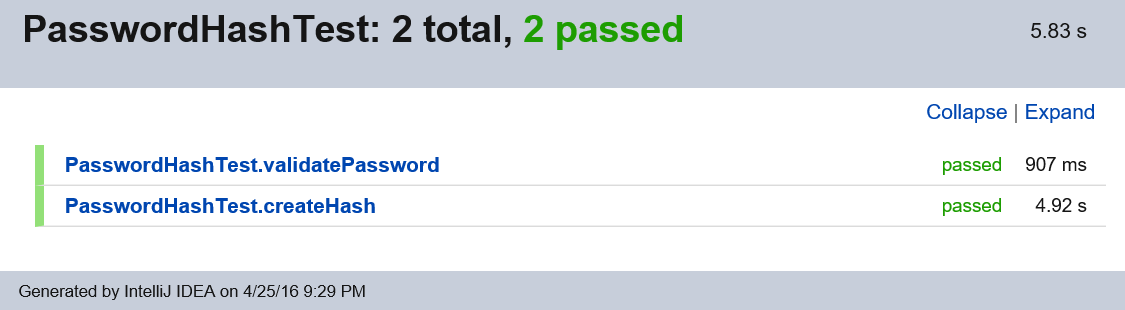
\includegraphics[width=\textwidth]{PasswordHashTest} \\ \\

This passed test indicates that we our hashing algorithm successfully validates a user's entered password with their hashed password, and properly creates non-colliding hashes. It also shows us that the createHash method takes 5 seconds to run, indicating a possible place for better optimization.

\begin{table}[h]
	\centering
	\caption{EditorControllerTest (dani2918)}
	\begin{tabular}{|p{3cm}|p{3cm}|p{9cm}|}
		\hline
		\textbf{Function Name} & \textbf{Result} & \textbf{Description}  \\\hline
		testSetupMobWrite() & FAILURE & Attempting to create a new CodeArea, which the setupMobWrite function requires as a parameter, was not working in the test class. Further investigation will be required to determine whether the function works properly.
		  \\\hline
	\end{tabular}
\end{table}


\begin{table}[h]
	\centering
	\caption{NewProjectControllerTest (dani2918)}
	\begin{tabular}{|p{3cm}|p{3cm}|p{9cm}|}
		\hline
		\textbf{Function Name} & \textbf{Result} & \textbf{Description}  \\\hline
		testInitProjectFields() & FAILURE & The test fails when attempting to create a project based upon the empty string as a title. We will have to implement logic to ensure that a user enters a project title in the appropriate field. This is the only case of those tested which caused a failure.
		  \\\hline
		  testCopyMainFile() & PASS & The copied file existed with multiple attempts.
		  \\\hline
	\end{tabular}
\end{table}

\newpage

\section{GUI Testing}

This section governs our GUI unit tests and the required output deemed as a ``pass''. Since we are using the JavaFX framework, every test case requires an initialization step of loading the .fxml file for the GUI scene to be tested. Once it is loaded we perform tests on individual parts of the scene using the TestFX libraries that integrate with JUnit.

\subsection{Test Classes}

\begin{table}[h]
	\centering	
	\caption{HomeTest (wern0096)}
	\begin{tabular}{|p{4cm}|p{5cm}|p{6cm}|} 
		\hline
		\textbf{Function Name} & \textbf{Description} & \textbf{Pass Criteria}  \\\hline
		verifyUiElementsLoaded() & Checks that every UI element loaded properly. & No exceptions thrown by the verifyThat$\left(\right)$ function calls. \\\hline
	\end{tabular}
\end{table}

\begin{table}[h]
	\centering	
	\caption{EditorTest (wern0096)}
	\begin{tabular}{|p{4cm}|p{5cm}|p{6cm}|} 
		\hline
		\textbf{Function Name} & \textbf{Description} & \textbf{Pass Criteria}  \\\hline
		verifyUiElementsLoaded() & Checks that every UI element loaded properly. & No exceptions thrown by the verifyThat$\left(\right)$ function calls. \\\hline
	\end{tabular}
\end{table}

\begin{table}[h]
	\centering
	\caption{NewProjectTest (dani2918)}
	\begin{tabular}{|p{4cm}|p{5cm}|p{6cm}|}
		\hline
		\textbf{Function Name} & \textbf{Description} & \textbf{Pass Criteria}  \\\hline
		verifyUiElementsLoaded() & Checks that every UI element loaded properly. & No exceptions thrown by the verifyThat$\left(\right)$ function calls. \\\hline
	\end{tabular}
\end{table}

\newpage
\subsection{Results}

\subsubsection{HomeTest}

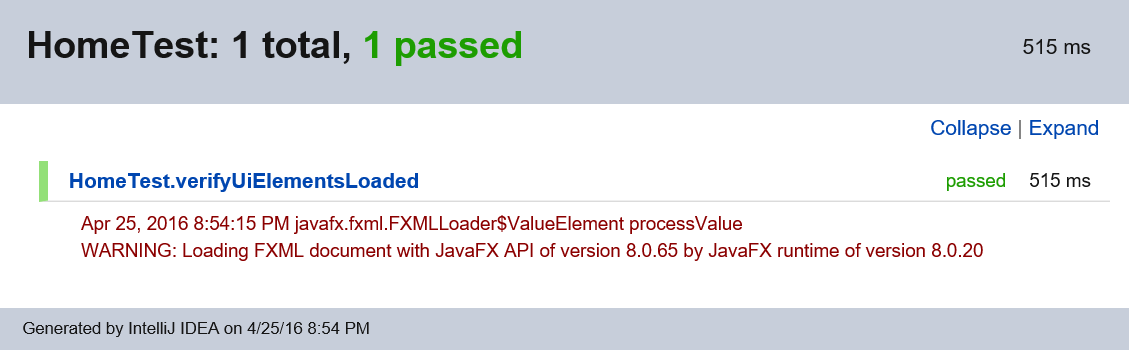
\includegraphics[width=\textwidth]{HomeTest} \\ \\

This passed test indicates that all UI elements are loading properly. It does create a warning message about a mismatch of the JavaFX API and the runtime, however, and wee will remedy that next sprint.

\newpage
\subsubsection{EditorTest}

\noindent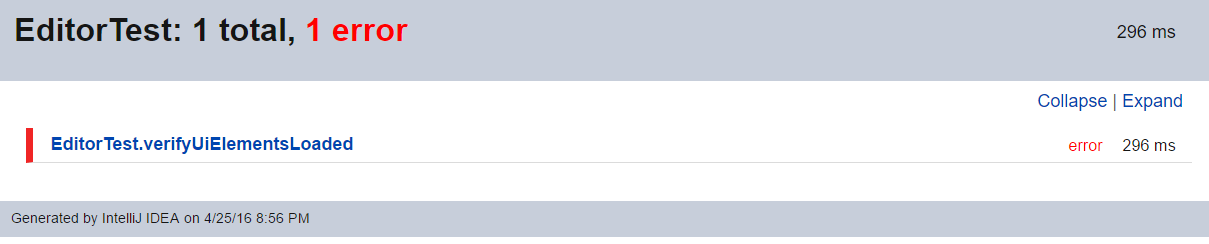
\includegraphics[width=\textwidth]{EditorTest} \\

This test currently fails due to it requiring initialization with data from another class. This will be better tested with an automation script, but it is still useful to know what data it requires to successfully initialize. Here is the following exception it throws:

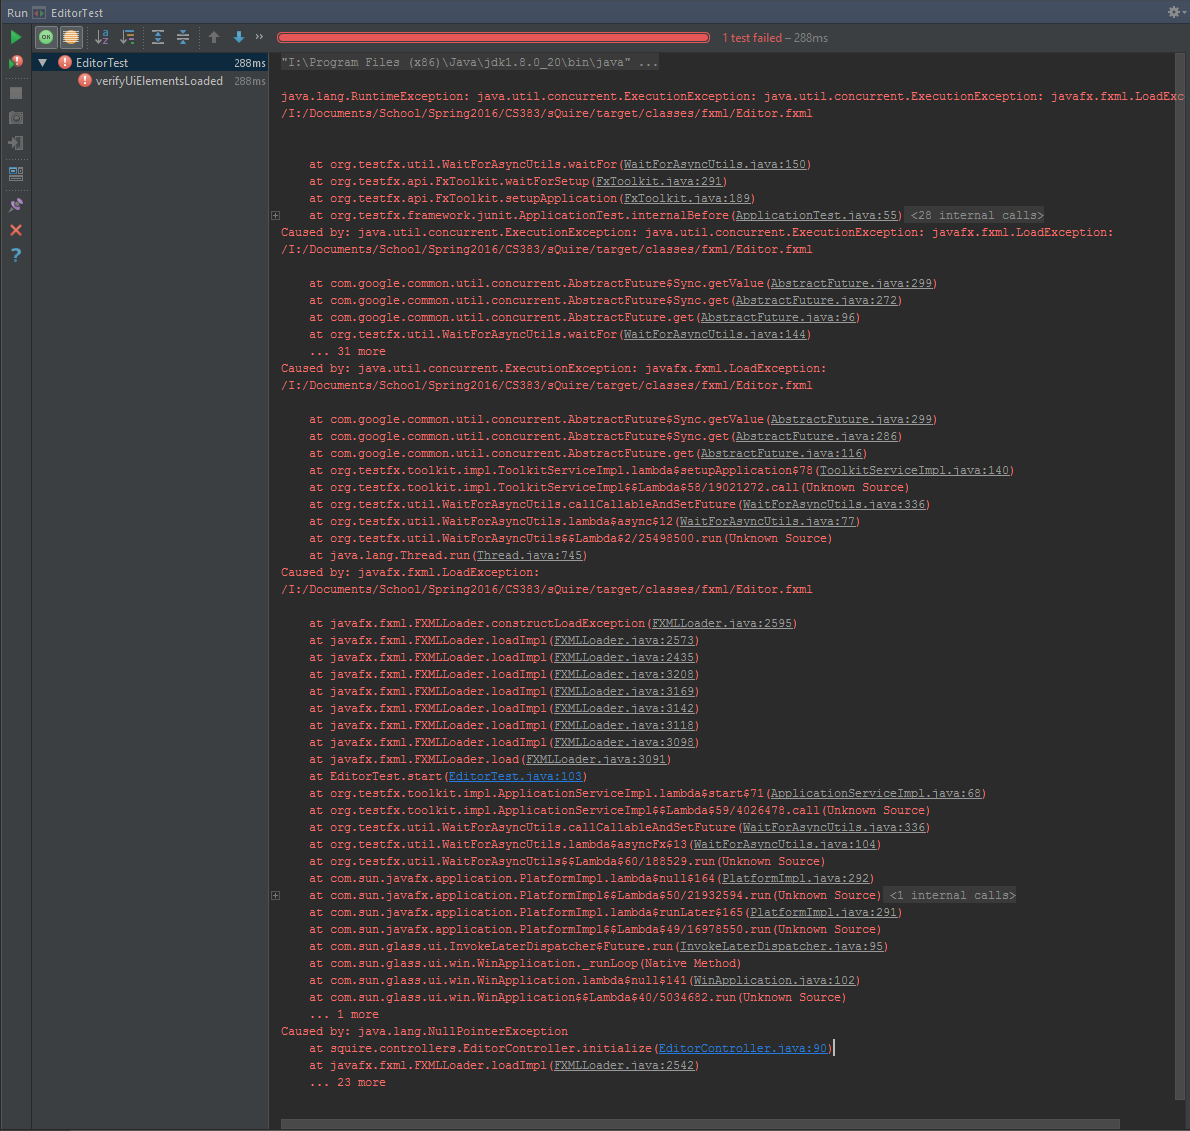
\includegraphics[width=\textwidth]{EditorTestException} 

\begin{table}[h]
	\centering
	\caption{NewProjectTest (dani2918)}
	\begin{tabular}{|p{5cm}|p{3cm}|p{4cm}|}
		\hline
		\textbf{Function Name} & \textbf{Description} & \textbf{Pass Criteria}  \\\hline
		verifyUiElementsLoaded() & PASS & No exceptions were thrown after loading all elements from the FXML file. \\\hline
	\end{tabular}
\end{table}


\newpage
\section{Back-end Testing}

This section governs any tests aimed at our database(s) or server(s) and the required output deemed as a ``pass''. \\

\subsection{Test Classes}

\begin{table}[h]
	\centering
	\caption{MobWriteClientTest (ratc8795)}
	\begin{tabular}{|p{4cm}|p{5cm}|p{6cm}|}
		\hline
		\textbf{Function Name} & \textbf{Description} & \textbf{Pass Criteria}  \\\hline
		%verifyUiElementsLoaded() & Checks that every UI element loaded properly. & No exceptions thrown by the verifyThat$\left(\right)$ function calls. \\\hline
	\end{tabular}
\end{table}
\begin{table}[h]
	\centering
	\caption{MobWriteServerTest (ratc8795)}
	\begin{tabular}{|p{4cm}|p{5cm}|p{6cm}|}
		\hline
		\textbf{Function Name} & \textbf{Description} & \textbf{Pass Criteria}  \\\hline
		%verifyUiElementsLoaded() & Checks that every UI element loaded properly. & No exceptions thrown by the verifyThat$\left(\right)$ function calls. \\\hline
	\end{tabular}
\end{table}
\begin{table}[h]
	\centering
	\caption{SessionTest (ratc8795)}
	\begin{tabular}{|p{4cm}|p{5cm}|p{6cm}|}
		\hline
		\textbf{Function Name} & \textbf{Description} & \textbf{Pass Criteria}  \\\hline
		%verifyUiElementsLoaded() & Checks that every UI element loaded properly. & No exceptions thrown by the verifyThat$\left(\right)$ function calls. \\\hline
	\end{tabular}
\end{table}
\begin{table}[h]
	\centering
	\caption{UserTest (ratc8795)}
	\begin{tabular}{|p{4cm}|p{5cm}|p{6cm}|}
		\hline
		\textbf{Function Name} & \textbf{Description} & \textbf{Pass Criteria}  \\\hline
		%verifyUiElementsLoaded() & Checks that every UI element loaded properly. & No exceptions thrown by the verifyThat$\left(\right)$ function calls. \\\hline
	\end{tabular}
\end{table}


\begin{table}[h]
	\centering
	\caption{ProjectDatabaseTest (cart1189)}
	\begin{tabular}{|p{4cm}|p{5cm}|p{6cm}|}
		\hline
		\textbf{Function Name} & \textbf{Description} & \textbf{Pass Criteria}  \\\hline
		testAddProject() & Checks the ability to create and save new Project objects to their database table. & No exceptions thrown during Project initialization or database save(). The new Project entry is in the table during the test. \\\hline
		testRemoveProject() & Checks the ability to remove Project object entries from their database table. & No exceptions thrown during Project initialization or database save(). The Project in question is removed from the table by the the end of the test. \\\hline
		testGetSetTextFields() & Checks ability to set each string field of a Project database entry, and retrieve those fields from the database. & No exceptions thrown by the test. Each retrieved value matches the value it was set to. \\\hline
		%func() & Desc & No exceptions thrown by the verifyThat$\left(\right)$ function calls. \\\hline
		%func() & Desc & No exceptions thrown by the verifyThat$\left(\right)$ function calls. \\\hline
	\end{tabular}
\end{table}

\begin{table}[h]
	\centering
	\caption{ChatServerTest (gent7104)}
	\begin{tabular}{|p{4cm}|p{5cm}|p{6cm}|}
		\hline
		\textbf{Function Name} & \textbf{Description} & \textbf{Pass Criteria}  \\\hline
		VerifyConnection() & Verify that the a connection has been made & No exception is thrown when testconnection() is called. \\\hline
	\end{tabular}
\end{table}

\begin{table}[h]
	\centering
	\caption{ChatClientTest (gent7104)}
	\begin{tabular}{|p{4cm}|p{5cm}|p{6cm}|}
		\hline
		\textbf{Function Name} & \textbf{Description} & \textbf{Pass Criteria}  \\\hline
		VerifySocektConnection() & Verify that the client was able to connect with the specified host and and port number & No exception is thrown when connecting to the socket. \\\hline
	\end{tabular}
\end{table}

\newpage

\subsection{Results}

The result of these tests should go here.

\newpage

\section{Coverage Testing (wern0096)}

\subsection{Methodology}

The coverage test of sQuire was performed by running the program with the coverage testing option enabled in IntelliJ IDEA and a developer manually navigating through all of the functionality in the program.

\subsection{Results}

The following report was then generated, showing usability per package: \\ \\

\noindent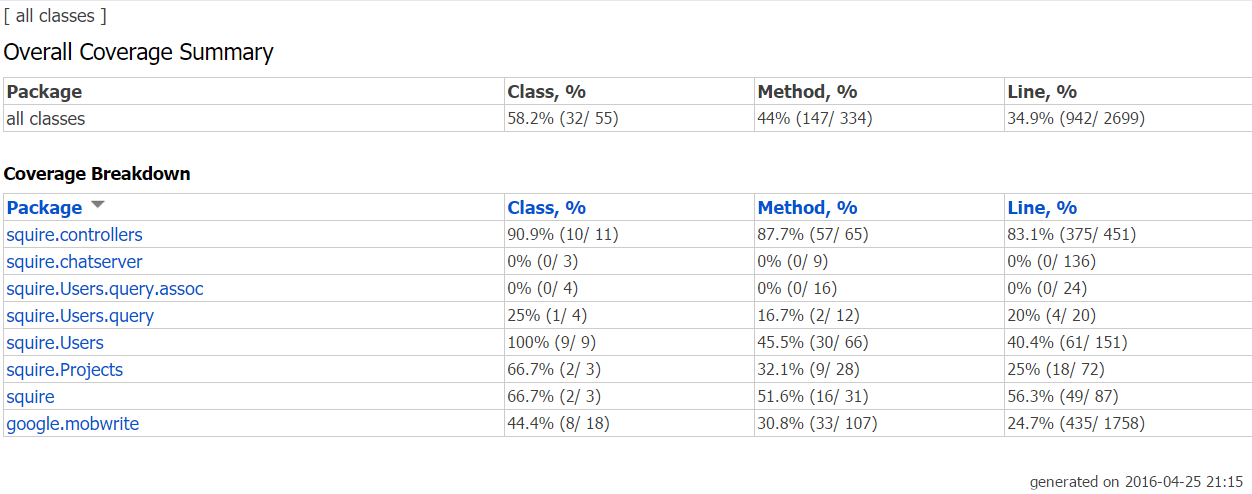
\includegraphics[width=\textwidth]{CoverageTest}

As indicated, most of the squire.controllers package was hit by our coverage test, indicating very little extraneous UI code. The chat server was not tested with this run, and the rest of the packages had about half of their functionalities hit, due to being heavily in development at the moment. As an example of the granularity of this report, let's examine the squire.controllers package to see what code didn't run during this test: \\ \\

\noindent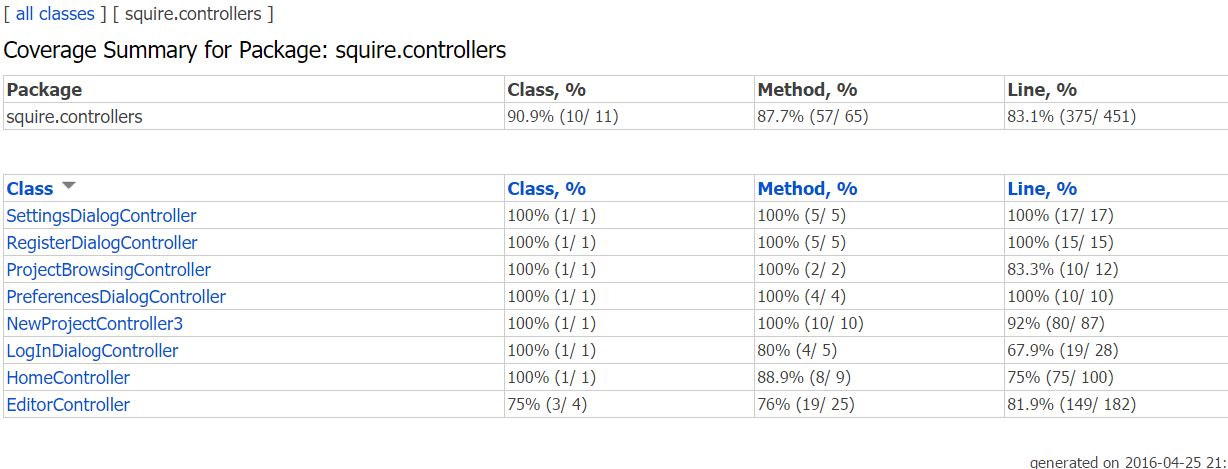
\includegraphics[width=\textwidth]{ControllerCoverageTest}

\noindent Delving further, let's see what code in the EditorController didn't run: \\ \\

\noindent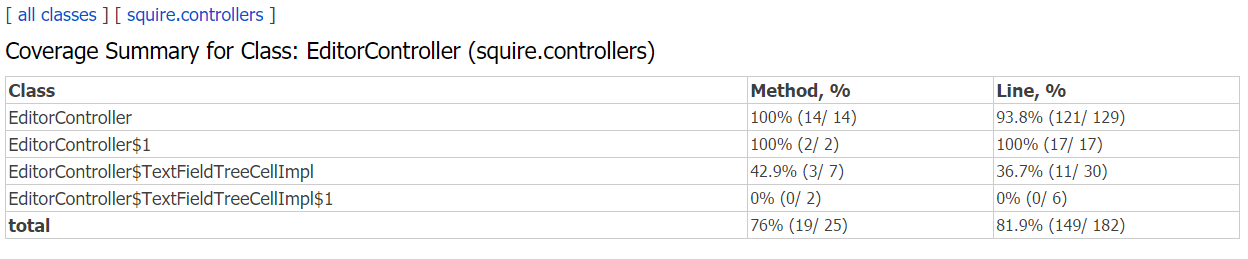
\includegraphics[width=\textwidth]{EditorControllerCoverage} \\ \\

\noindent Lastly, we can get very granular and see exactly which lines of code didn't run. Here's an example of the updateItem() function's code and how the IntelliJ Coverage Report displays code that was hit with a green outline and code that wasn't hit with a red outline: \\ \\

\noindent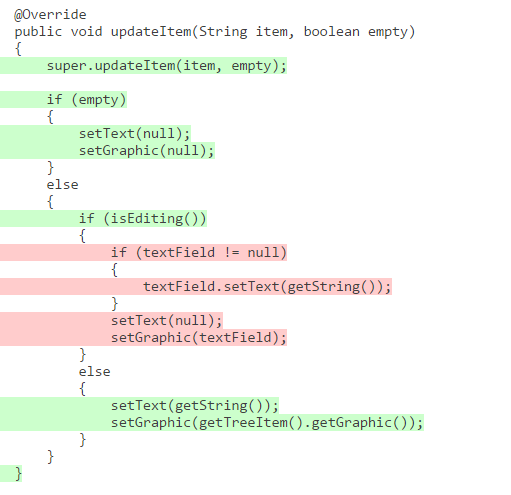
\includegraphics[scale=0.7]{EditorControllerCoverageFunction}


\newpage
\section{Software Risk Issues (wern0096)}

\subsection{High Risk}

The following items are deemed high risk to the security of users and to the usability and quality of the sQuire software:

\begin{itemize}
	\item \textbf{MobWrite Server and Client} \\ \\
	Our collaborative editing relies on Google's MobWrite software library. We are rating it high risk because it is the core of the collaborative editing functionality, and it is also a third-party tool with a high impact on the functionality of our product. This module also incorporates the diff-match-patch algorithm running on clients' machines that talks to our Azure server that broadcasts text changes from one client to the rest of the clients. Since it will be sending code over the internet to and from the server, the security implications for all machines involved are very serious. As such, we plan to have extensive testing and review of code using this module.
	\item \textbf{Chat Client} \\ \\
	Our chat client is simply a Java application running indefinitely in the same Azure server as the MobWrite server. Nevertheless, it is broadcasting possibly confidential data through the internet and should have the proper encryption and security reviews as the rest of the high risk items.
	\item \textbf{JavaFX} \\ \\
	The JavaFX framework is also core to our program. Since it has been used to build most of the user interface, it will require great usability and coverage testing to make sure that it is friendly and intuitive to our users. The breakdown of the user interface would essentially render the rest of the program useless. Thus, it receives a high risk rating.
	\item \textbf{Database Credentials} \\ \\
	The project uses a SQLite database for storing of user credentials and project information. We rate the security of user and project credentials in the database as high risk. In order to protect the confidentiality of user credentials and integrity of user projects, we will have to adhere to database security best practices such as salting and hashing stored credentials, encrypting traffic over the internet, and ensuring SQL-injection attacks are mitigated.
\end{itemize}

\subsection{Medium Risk}

The following items are deemed medium risk to the security of users and to the usability and quality of the sQuire software:

\begin{itemize}
	\item \textbf{Database Storage and Ebean ORM} \\ \\
	The non-confidential data stored in the database is rated as medium risk. This is because project data is also stored locally, and breakdown of the database storage functionality would not severely reduce core functionality of the sQuire software. However, it would still significantly hinder collaborative functionality. To address this, we plan on extensively testing database commands with unit tests and code reviews.
	
	\item \textbf{Code Compilation} \\ \\
	Whenever code compilation is involved, security becomes a concern. However, there is not code being executed remotely, so the security risks become much smaller, thus earning this module a medium rating. Compilation in sQuire will rely on the user reviewing their code for malicious intent before executing. We plan on implementing tools for the user to easily track changes to the code in order to aid in the review process if we have time. Also, we will have unit tests making sure that the user is properly notified of code errors and their location(s).
	
	\item \textbf{Testing Modules} \\ \\
	We are putting testing modules themselves as a medium risk item because of the sheer complexity of testing the user interface with JavaFX and TestFX, another open source framework. Since the user interface is rated as a high-risk item, we believe that properly testing it is at least a medium risk item to the proper functionality of our program. We didn't rate it as high-risk, because there are many ways of testing the user interface that are less complex but take more time.
\end{itemize}

\subsection{Low Risk}

The following items are deemed low risk to the security of users and to the usability and quality of the sQuire software:

\begin{itemize}
	\item \textbf{Editor Features} \\ \\
	This module features some complicated code that will come from third-party open sources such as search/replace, syntax highlighting, and auto-complete. However, failure of this module does not severely endanger users' security or the core functionality of the software. As such, it earns a low risk rating. This module will require extensive unit testing, however.
	\item \textbf{Local File Structure} \\ \\
	The local file structure stores user's projects locally in the form of a folder for each project. We rate this module as a low risk module because even if the local files were corrupted or deleted, the user's projects/files can still be restored from the database, and the program has code to handle such a case. Nevertheless, we plan to have various unit tests documenting valid/invalid file structures that we can then create code to handle such cases.
	\item \textbf{Program Settings} \\ \\
	This module involves settable user preferences that should persist between runs of sQuire. We plan to have the user's settings be saved locally as well as on the database, so that upon login, sQuire will update to conform to the user's preferences. Since there is redundancy to this module and its breakdown does not constitute a large hit to the functionality of sQuire, we deem it low risk.
\end{itemize}

\end{document}